%!TEX root = ../Main.tex

\chapter{研究一}\label{ch-name}
\section{引言}

\section{模块一}\label{sec-feature}

\subsection{子模块}

详见表格\ref{tab:name}

\begin{table}[htbp]\footnotesize
	\bicaption{图xx征}{Ixatures}
	\label{tab:name}
    \begin{tabular}{p{1cm}llp{9.3cm}}
		\hline
		\rowcolor{gray!15}
		\textbf{类别}                   & \textbf{特征}             & \textbf{维度} & \textbf{概述}                                              \\ \hline
		\multirow{4}{*}{颜色}              & HSxx          & 5          & H通道xx准差 \\
		& 颜色xx             & 3          & Valxx量                           \\
		& 颜xx          & 1          & 到均一xxe,xx)                                                                                    \\
		& 颜色xx例                & 11         & 黑色xx色和黄色的占比                                                \\
		\hline
		\multirow{4}{*}{xxx图}        & xx素               & 1          & Caxx素的比例                           \\
		& 细xxx           & 2          & Meaxx率                                                                              \\
		& 浅xx标  & 3          & 图像xx度                                            \\
		& 三xx则            & 2          & 图像xx                                                  \\
		\hline
		\multirow{5}{*}{纹xx} & xxx & 1          & 图xx熵                                                           \\
		& xx理    & 12         & 通过Daubss度水平                                     \\
		& xx纹理                    & 3          & 粗xx方向性的量                                            \\
		& Gxx理           & 12         & 每个Hxx匀性的量                                       \\
		 & GIxx理          & 24         & 用于xx输出                                       \\ 
		\hline
		% \cline{2-4} 
	\end{tabular}
\end{table}
\vspace{-10pt}

具体流程见算法\ref{alg:name}。

\begin{algorithm}\small
	\caption{计xx类别比例}\label{alg:name}
	\begin{algorithmic}[1]
		\REQUIRE 图像,存储在\texttt{bgr\_img}中;颜色xx,存储在\texttt{"color\_dict.npz"}中
		\ENSURE 图像中每xx分比列表
		
		\STATE // 统计xx次
		\STATE 加xx典\texttt{"color\_dict.npz"}至\texttt{color\_dict}
		\STATE 将\texttt{bgr\_img}从xx格式
		\STATE 将Rxx除以8
		\STATE 将xxxx通道
		\STATE 对于每个像素,计算唯一键:\texttt{unique\_key = red * (32 * 32) + green * 32 + blue}
		\STATE // 计算图xx分比
		\STATE 使用\texttt{unique\_key}从\texttt{color\_dict}中xx频率
		\STATE 计算xx度(\texttt{h})和宽度(\texttt{w})
		\STATE 对图xx,并除以h·w
		\STATE 返回xx列表
	\end{algorithmic}
\end{algorithm}


\begin{table}[h!]\small%[htbp]\small
	\centering
	\begin{threeparttable}[b]
		\bicaption{人脸x表}{InventoryxMBTxality}
		\label{tbl:dataset survey}
		\begin{tabular}{|c|p{7.4cm}|p{5cm}|} 
			\hline
			\rowcolor{gray!15}
			序号 & 原xx题 & 问题翻译 \\
			\hline
			1 & Pleasxxe. & 请上传一xx活照。 \\  
			\hline
			2 & Please xxe test\tnote{*} and uploadxxt result. & 请做xx果截图。\\
			\hline  
			3 & Please select your pxxnt test. & 请根据xx类型.\\
			\hline
			4 & Is the resxxicable". & 本次测xx合”。\\  
			\hline
		\end{tabular}
		\begin{tablenotes}
			\footnotesize
			\item[*] 16perxersonality-test。
		\end{tablenotes}
	\end{threeparttable}
\end{table}



\begin{table}[ht]\footnotesize
	\centering
	\bicaption{Mxx计信息}{MBxxtistics}
	\label{tbl:text-dataset-stats}
	\begin{tabular}{c|c||ccc}
		\hline%\toprule
		\rowcolor{gray!15}
		数据集 & 人xx质 & 训练集 (60\%) & 验证集 (20\%) & 测试集 (20\%) \\
		\hline%\midrule
		\multirow{4}{*}{Mxxk} & xx & 4x8 / 11x2 & 14x/ 38x6 & 143x7 / x77 \\
		& xx & 7xx / 48xx& x / 1x5 & 2x/ 16x\\
		& xx & 3xx9 / 1xx1 & 11xx0 / 6x3 & 11x2 / x2 \\
		& xx & 3xx1 / 2xx9 & 10x3 / x0 & x6 / 7x8 \\
		\hline%\addlinespace
		\multirow{4}{*}{Kaxe} & x & 40x/ 1x4 & 1x6 / 4x & 1x9 / x6 \\
		& x & 6x/ 4478 & x2 / x & x8 / 1x\\
		& x & 24x0 / 2x95 & 7x1 / 9x4 & 78x/ x5 \\
		& Jx & 3x96 / 2x09 & 10x3 / x2 & 10x / x3 \\
		\hline%\bottomrule
	\end{tabular}
\end{table}




\vspace{20pt}

\begin{footnotesize}
\begin{longtable}{|l||c|c|c|c|c||c|c|c|c|}
	\bicaption{视觉x系数}{Spexsoxraits}
	\label{tab:xon}\\%这里的换行符号一定要有!!!去掉会报错的
	
	% 首页的表头
	\hline%	\thickhline
	\rowcolor{gray!15} \textbf{特征} & \multicolumn{5}{c||}{\textbf{大x格}} & \multicolumn{4}{c|}{\textbf{Mx}} \\

%	\hline%\thickhline
	\hhline{*{10}{:=}:}%\thickhline
	\rowcolor{gray!15} \textbf{颜色} & \textbf{Ox} & \textbf{Cxn} & \textbf{x} & \textbf{xr} & \textbf{xu} & \textbf{I} & \textbf{N} & \textbf{F} & \textbf{J} \\
	\hhline{*{10}{:=}:}%\thickhline
	
	\endfirsthead
	
	%续表的表头
	
	%此命令用于控制续表标题的上行距
	\specialrule{0em}{0pt}{-8pt}%{8pt}%{11.06pt}
	
	\multicolumn{10}{c}{\biaozihao 续表 \ref{tab:xon}\ \ \ \ 视觉x与x数\vspace{5pt}}\\	
	\multicolumn{10}{c}{\biaozihaoeng Table \ref{tab:xon}\ \ \ \ Spxts }\\%(continued)}\\	
	
	%此命令用于控制续表标题的下行距
	\specialrule{0em}{0pt}{5pt}%{5.03pt}
	
	% 续表的表头具体内容
	
	\hline%\thickhline
	\rowcolor{gray!15} \textbf{特征} & \multicolumn{5}{c||}{\textbf{x人格}} & \multicolumn{4}{c|}{\textbf{xI}} \\

	\hhline{*{10}{:=}:}%\thickhline
	\rowcolor{gray!15} \textbf{x理} & \textbf{Ox} & \textbf{xon} & \textbf{Ex} & \textbf{xr} & \textbf{Nx} & \textbf{E} & \textbf{N} & \textbf{F} & \textbf{P} \\
	\hline%\thickhline
	
	\endhead
	
	% 表底
	\hline%\thickhline
	\endfoot
	
	\hline%\thickhline
	\endlastfoot
	\hline
	色x(H) & \colorForValue{-0.203} -0.203 & \colorForValue{-0.15} -0.15 & \colorForValue{0.077} 0.077 & \colorForValue{-0.068} -0.068 & \colorForValue{0.537} 0.537 & \colorForValue{-0.038} -0.038 & \colorForValue{-0.032} -0.032 & \colorForValue{-0.073} -0.073 & \colorForValue{-0.061} -0.061 \\
	\hline
	色x(H) & \colorForValue{-0.203} -0.203 & \colorForValue{-0.15} -0.15 & \colorForValue{0.077} 0.077 & \colorForValue{-0.068} -0.068 & \colorForValue{0.537} 0.537 & \colorForValue{-0.038} -0.038 & \colorForValue{-0.032} -0.032 & \colorForValue{-0.073} -0.073 & \colorForValue{-0.061} -0.061 \\
	\hline
	色x(H) & \colorForValue{-0.203} -0.203 & \colorForValue{-0.15} -0.15 & \colorForValue{0.077} 0.077 & \colorForValue{-0.068} -0.068 & \colorForValue{0.537} 0.537 & \colorForValue{-0.038} -0.038 & \colorForValue{-0.032} -0.032 & \colorForValue{-0.073} -0.073 & \colorForValue{-0.061} -0.061 \\
	\hline
	色x(H) & \colorForValue{-0.203} -0.203 & \colorForValue{-0.15} -0.15 & \colorForValue{0.077} 0.077 & \colorForValue{-0.068} -0.068 & \colorForValue{0.537} 0.537 & \colorForValue{-0.038} -0.038 & \colorForValue{-0.032} -0.032 & \colorForValue{-0.073} -0.073 & \colorForValue{-0.061} -0.061 \\
	\hline
	色x(H) & \colorForValue{-0.203} -0.203 & \colorForValue{-0.15} -0.15 & \colorForValue{0.077} 0.077 & \colorForValue{-0.068} -0.068 & \colorForValue{0.537} 0.537 & \colorForValue{-0.038} -0.038 & \colorForValue{-0.032} -0.032 & \colorForValue{-0.073} -0.073 & \colorForValue{-0.061} -0.061 \\
	\hline
	色x(H) & \colorForValue{-0.203} -0.203 & \colorForValue{-0.15} -0.15 & \colorForValue{0.077} 0.077 & \colorForValue{-0.068} -0.068 & \colorForValue{0.537} 0.537 & \colorForValue{-0.038} -0.038 & \colorForValue{-0.032} -0.032 & \colorForValue{-0.073} -0.073 & \colorForValue{-0.061} -0.061 \\
	\hline
	色x(H) & \colorForValue{-0.203} -0.203 & \colorForValue{-0.15} -0.15 & \colorForValue{0.077} 0.077 & \colorForValue{-0.068} -0.068 & \colorForValue{0.537} 0.537 & \colorForValue{-0.038} -0.038 & \colorForValue{-0.032} -0.032 & \colorForValue{-0.073} -0.073 & \colorForValue{-0.061} -0.061 \\
	\hline
	色x(H) & \colorForValue{-0.203} -0.203 & \colorForValue{-0.15} -0.15 & \colorForValue{0.077} 0.077 & \colorForValue{-0.068} -0.068 & \colorForValue{0.537} 0.537 & \colorForValue{-0.038} -0.038 & \colorForValue{-0.032} -0.032 & \colorForValue{-0.073} -0.073 & \colorForValue{-0.061} -0.061 \\
	\hline
	色x(H) & \colorForValue{-0.203} -0.203 & \colorForValue{-0.15} -0.15 & \colorForValue{0.077} 0.077 & \colorForValue{-0.068} -0.068 & \colorForValue{0.537} 0.537 & \colorForValue{-0.038} -0.038 & \colorForValue{-0.032} -0.032 & \colorForValue{-0.073} -0.073 & \colorForValue{-0.061} -0.061 \\
	\hline
	色x(H) & \colorForValue{-0.203} -0.203 & \colorForValue{-0.15} -0.15 & \colorForValue{0.077} 0.077 & \colorForValue{-0.068} -0.068 & \colorForValue{0.537} 0.537 & \colorForValue{-0.038} -0.038 & \colorForValue{-0.032} -0.032 & \colorForValue{-0.073} -0.073 & \colorForValue{-0.061} -0.061 \\
	\hline
	色x(H) & \colorForValue{-0.203} -0.203 & \colorForValue{-0.15} -0.15 & \colorForValue{0.077} 0.077 & \colorForValue{-0.068} -0.068 & \colorForValue{0.537} 0.537 & \colorForValue{-0.038} -0.038 & \colorForValue{-0.032} -0.032 & \colorForValue{-0.073} -0.073 & \colorForValue{-0.061} -0.061 \\
	\hline
	色x(H) & \colorForValue{-0.203} -0.203 & \colorForValue{-0.15} -0.15 & \colorForValue{0.077} 0.077 & \colorForValue{-0.068} -0.068 & \colorForValue{0.537} 0.537 & \colorForValue{-0.038} -0.038 & \colorForValue{-0.032} -0.032 & \colorForValue{-0.073} -0.073 & \colorForValue{-0.061} -0.061 \\
	\hline
	色x(H) & \colorForValue{-0.203} -0.203 & \colorForValue{-0.15} -0.15 & \colorForValue{0.077} 0.077 & \colorForValue{-0.068} -0.068 & \colorForValue{0.537} 0.537 & \colorForValue{-0.038} -0.038 & \colorForValue{-0.032} -0.032 & \colorForValue{-0.073} -0.073 & \colorForValue{-0.061} -0.061 \\
	\hline
	色x(H) & \colorForValue{-0.203} -0.203 & \colorForValue{-0.15} -0.15 & \colorForValue{0.077} 0.077 & \colorForValue{-0.068} -0.068 & \colorForValue{0.537} 0.537 & \colorForValue{-0.038} -0.038 & \colorForValue{-0.032} -0.032 & \colorForValue{-0.073} -0.073 & \colorForValue{-0.061} -0.061 \\
	\hline
	色x(H) & \colorForValue{-0.203} -0.203 & \colorForValue{-0.15} -0.15 & \colorForValue{0.077} 0.077 & \colorForValue{-0.068} -0.068 & \colorForValue{0.537} 0.537 & \colorForValue{-0.038} -0.038 & \colorForValue{-0.032} -0.032 & \colorForValue{-0.073} -0.073 & \colorForValue{-0.061} -0.061 \\
	\hline
	色x(H) & \colorForValue{-0.203} -0.203 & \colorForValue{-0.15} -0.15 & \colorForValue{0.077} 0.077 & \colorForValue{-0.068} -0.068 & \colorForValue{0.537} 0.537 & \colorForValue{-0.038} -0.038 & \colorForValue{-0.032} -0.032 & \colorForValue{-0.073} -0.073 & \colorForValue{-0.061} -0.061 \\
	\hline
	色x(H) & \colorForValue{-0.203} -0.203 & \colorForValue{-0.15} -0.15 & \colorForValue{0.077} 0.077 & \colorForValue{-0.068} -0.068 & \colorForValue{0.537} 0.537 & \colorForValue{-0.038} -0.038 & \colorForValue{-0.032} -0.032 & \colorForValue{-0.073} -0.073 & \colorForValue{-0.061} -0.061 \\
	\hline
	色x(H) & \colorForValue{-0.203} -0.203 & \colorForValue{-0.15} -0.15 & \colorForValue{0.077} 0.077 & \colorForValue{-0.068} -0.068 & \colorForValue{0.537} 0.537 & \colorForValue{-0.038} -0.038 & \colorForValue{-0.032} -0.032 & \colorForValue{-0.073} -0.073 & \colorForValue{-0.061} -0.061 \\
	\hline
	色x(H) & \colorForValue{-0.203} -0.203 & \colorForValue{-0.15} -0.15 & \colorForValue{0.077} 0.077 & \colorForValue{-0.068} -0.068 & \colorForValue{0.537} 0.537 & \colorForValue{-0.038} -0.038 & \colorForValue{-0.032} -0.032 & \colorForValue{-0.073} -0.073 & \colorForValue{-0.061} -0.061 \\
	\hline
	色x(H) & \colorForValue{-0.203} -0.203 & \colorForValue{-0.15} -0.15 & \colorForValue{0.077} 0.077 & \colorForValue{-0.068} -0.068 & \colorForValue{0.537} 0.537 & \colorForValue{-0.038} -0.038 & \colorForValue{-0.032} -0.032 & \colorForValue{-0.073} -0.073 & \colorForValue{-0.061} -0.061 \\
	\hhline{*{10}{:=}:}%\thickhline
	\rowcolor{gray!15} \textbf{构x} & \textbf{Ope} & \textbf{Con} & \textbf{Ext} & \textbf{Agr} & \textbf{Neu} & \textbf{I} & \textbf{N} & \textbf{T} & \textbf{J} \\
	\hhline{*{10}{:=}:}%\thickhline
	边x & \colorForValue{-0.371} -0.371 & \colorForValue{0.127} 0.127 & \colorForValue{-0.414} -0.414 & \colorForValue{0.383} 0.383 & \colorForValue{0.338} 0.338 & \colorForValue{0.076} 0.076 & \colorForValue{-0.102} -0.102 & \colorForValue{-0.474} -0.474 & \colorForValue{-0.227} -0.227 \\
	\hline
	边x & \colorForValue{-0.371} -0.371 & \colorForValue{0.127} 0.127 & \colorForValue{-0.414} -0.414 & \colorForValue{0.383} 0.383 & \colorForValue{0.338} 0.338 & \colorForValue{0.076} 0.076 & \colorForValue{-0.102} -0.102 & \colorForValue{-0.474} -0.474 & \colorForValue{-0.227} -0.227 \\
	\hline
	边x & \colorForValue{-0.371} -0.371 & \colorForValue{0.127} 0.127 & \colorForValue{-0.414} -0.414 & \colorForValue{0.383} 0.383 & \colorForValue{0.338} 0.338 & \colorForValue{0.076} 0.076 & \colorForValue{-0.102} -0.102 & \colorForValue{-0.474} -0.474 & \colorForValue{-0.227} -0.227 \\
	\hline
	边x & \colorForValue{-0.371} -0.371 & \colorForValue{0.127} 0.127 & \colorForValue{-0.414} -0.414 & \colorForValue{0.383} 0.383 & \colorForValue{0.338} 0.338 & \colorForValue{0.076} 0.076 & \colorForValue{-0.102} -0.102 & \colorForValue{-0.474} -0.474 & \colorForValue{-0.227} -0.227 \\
	\hline
	边x & \colorForValue{-0.371} -0.371 & \colorForValue{0.127} 0.127 & \colorForValue{-0.414} -0.414 & \colorForValue{0.383} 0.383 & \colorForValue{0.338} 0.338 & \colorForValue{0.076} 0.076 & \colorForValue{-0.102} -0.102 & \colorForValue{-0.474} -0.474 & \colorForValue{-0.227} -0.227 \\
	\hline
	边x & \colorForValue{-0.371} -0.371 & \colorForValue{0.127} 0.127 & \colorForValue{-0.414} -0.414 & \colorForValue{0.383} 0.383 & \colorForValue{0.338} 0.338 & \colorForValue{0.076} 0.076 & \colorForValue{-0.102} -0.102 & \colorForValue{-0.474} -0.474 & \colorForValue{-0.227} -0.227 \\
	\hline
	边x & \colorForValue{-0.371} -0.371 & \colorForValue{0.127} 0.127 & \colorForValue{-0.414} -0.414 & \colorForValue{0.383} 0.383 & \colorForValue{0.338} 0.338 & \colorForValue{0.076} 0.076 & \colorForValue{-0.102} -0.102 & \colorForValue{-0.474} -0.474 & \colorForValue{-0.227} -0.227 \\
	\hline
	边x & \colorForValue{-0.371} -0.371 & \colorForValue{0.127} 0.127 & \colorForValue{-0.414} -0.414 & \colorForValue{0.383} 0.383 & \colorForValue{0.338} 0.338 & \colorForValue{0.076} 0.076 & \colorForValue{-0.102} -0.102 & \colorForValue{-0.474} -0.474 & \colorForValue{-0.227} -0.227 \\
	\hhline{*{10}{:=}:}%\thickhline
	\rowcolor{gray!15} \textbf{xxx} & \textbf{Ope} & \textbf{Con} & \textbf{Ext} & \textbf{Agr} & \textbf{Neu} & \textbf{I} & \textbf{N} & \textbf{T} & \textbf{J} \\
	\hhline{*{10}{:=}:}%\thickhline
	x熵 & \colorForValue{-0.346} -0.346 & \colorForValue{0.498} 0.498 & \colorForValue{0.206} 0.206 & \colorForValue{-0.313} -0.313 & \colorForValue{0.492} 0.492 & \colorForValue{0.254} 0.254 & \colorForValue{-0.071} -0.071 & \colorForValue{-0.315} -0.315 & \colorForValue{-0.037} -0.037 \\
	\hline
	x熵 & \colorForValue{-0.346} -0.346 & \colorForValue{0.498} 0.498 & \colorForValue{0.206} 0.206 & \colorForValue{-0.313} -0.313 & \colorForValue{0.492} 0.492 & \colorForValue{0.254} 0.254 & \colorForValue{-0.071} -0.071 & \colorForValue{-0.315} -0.315 & \colorForValue{-0.037} -0.037 \\
	\hline
	x熵 & \colorForValue{-0.346} -0.346 & \colorForValue{0.498} 0.498 & \colorForValue{0.206} 0.206 & \colorForValue{-0.313} -0.313 & \colorForValue{0.492} 0.492 & \colorForValue{0.254} 0.254 & \colorForValue{-0.071} -0.071 & \colorForValue{-0.315} -0.315 & \colorForValue{-0.037} -0.037 \\
	\hline
	x熵 & \colorForValue{-0.346} -0.346 & \colorForValue{0.498} 0.498 & \colorForValue{0.206} 0.206 & \colorForValue{-0.313} -0.313 & \colorForValue{0.492} 0.492 & \colorForValue{0.254} 0.254 & \colorForValue{-0.071} -0.071 & \colorForValue{-0.315} -0.315 & \colorForValue{-0.037} -0.037 \\
	\hline
	x熵 & \colorForValue{-0.346} -0.346 & \colorForValue{0.498} 0.498 & \colorForValue{0.206} 0.206 & \colorForValue{-0.313} -0.313 & \colorForValue{0.492} 0.492 & \colorForValue{0.254} 0.254 & \colorForValue{-0.071} -0.071 & \colorForValue{-0.315} -0.315 & \colorForValue{-0.037} -0.037 \\
	\hline
	x熵 & \colorForValue{-0.346} -0.346 & \colorForValue{0.498} 0.498 & \colorForValue{0.206} 0.206 & \colorForValue{-0.313} -0.313 & \colorForValue{0.492} 0.492 & \colorForValue{0.254} 0.254 & \colorForValue{-0.071} -0.071 & \colorForValue{-0.315} -0.315 & \colorForValue{-0.037} -0.037 \\
	\hline
	x熵 & \colorForValue{-0.346} -0.346 & \colorForValue{0.498} 0.498 & \colorForValue{0.206} 0.206 & \colorForValue{-0.313} -0.313 & \colorForValue{0.492} 0.492 & \colorForValue{0.254} 0.254 & \colorForValue{-0.071} -0.071 & \colorForValue{-0.315} -0.315 & \colorForValue{-0.037} -0.037 \\
	\hline
	x熵 & \colorForValue{-0.346} -0.346 & \colorForValue{0.498} 0.498 & \colorForValue{0.206} 0.206 & \colorForValue{-0.313} -0.313 & \colorForValue{0.492} 0.492 & \colorForValue{0.254} 0.254 & \colorForValue{-0.071} -0.071 & \colorForValue{-0.315} -0.315 & \colorForValue{-0.037} -0.037 \\
	\hline
	x熵 & \colorForValue{-0.346} -0.346 & \colorForValue{0.498} 0.498 & \colorForValue{0.206} 0.206 & \colorForValue{-0.313} -0.313 & \colorForValue{0.492} 0.492 & \colorForValue{0.254} 0.254 & \colorForValue{-0.071} -0.071 & \colorForValue{-0.315} -0.315 & \colorForValue{-0.037} -0.037 \\
	\hline
	x熵 & \colorForValue{-0.346} -0.346 & \colorForValue{0.498} 0.498 & \colorForValue{0.206} 0.206 & \colorForValue{-0.313} -0.313 & \colorForValue{0.492} 0.492 & \colorForValue{0.254} 0.254 & \colorForValue{-0.071} -0.071 & \colorForValue{-0.315} -0.315 & \colorForValue{-0.037} -0.037 \\
	\hline
	x熵 & \colorForValue{-0.346} -0.346 & \colorForValue{0.498} 0.498 & \colorForValue{0.206} 0.206 & \colorForValue{-0.313} -0.313 & \colorForValue{0.492} 0.492 & \colorForValue{0.254} 0.254 & \colorForValue{-0.071} -0.071 & \colorForValue{-0.315} -0.315 & \colorForValue{-0.037} -0.037 \\
	\hline
	x熵 & \colorForValue{-0.346} -0.346 & \colorForValue{0.498} 0.498 & \colorForValue{0.206} 0.206 & \colorForValue{-0.313} -0.313 & \colorForValue{0.492} 0.492 & \colorForValue{0.254} 0.254 & \colorForValue{-0.071} -0.071 & \colorForValue{-0.315} -0.315 & \colorForValue{-0.037} -0.037 \\
	\hline
	x熵 & \colorForValue{-0.346} -0.346 & \colorForValue{0.498} 0.498 & \colorForValue{0.206} 0.206 & \colorForValue{-0.313} -0.313 & \colorForValue{0.492} 0.492 & \colorForValue{0.254} 0.254 & \colorForValue{-0.071} -0.071 & \colorForValue{-0.315} -0.315 & \colorForValue{-0.037} -0.037 \\
	\hline
	x熵 & \colorForValue{-0.346} -0.346 & \colorForValue{0.498} 0.498 & \colorForValue{0.206} 0.206 & \colorForValue{-0.313} -0.313 & \colorForValue{0.492} 0.492 & \colorForValue{0.254} 0.254 & \colorForValue{-0.071} -0.071 & \colorForValue{-0.315} -0.315 & \colorForValue{-0.037} -0.037 \\
	\hline
	x熵 & \colorForValue{-0.346} -0.346 & \colorForValue{0.498} 0.498 & \colorForValue{0.206} 0.206 & \colorForValue{-0.313} -0.313 & \colorForValue{0.492} 0.492 & \colorForValue{0.254} 0.254 & \colorForValue{-0.071} -0.071 & \colorForValue{-0.315} -0.315 & \colorForValue{-0.037} -0.037 \\
	\hline
	x熵 & \colorForValue{-0.346} -0.346 & \colorForValue{0.498} 0.498 & \colorForValue{0.206} 0.206 & \colorForValue{-0.313} -0.313 & \colorForValue{0.492} 0.492 & \colorForValue{0.254} 0.254 & \colorForValue{-0.071} -0.071 & \colorForValue{-0.315} -0.315 & \colorForValue{-0.037} -0.037 \\
	\hline
	x熵 & \colorForValue{-0.346} -0.346 & \colorForValue{0.498} 0.498 & \colorForValue{0.206} 0.206 & \colorForValue{-0.313} -0.313 & \colorForValue{0.492} 0.492 & \colorForValue{0.254} 0.254 & \colorForValue{-0.071} -0.071 & \colorForValue{-0.315} -0.315 & \colorForValue{-0.037} -0.037 \\
	\hline
	x熵 & \colorForValue{-0.346} -0.346 & \colorForValue{0.498} 0.498 & \colorForValue{0.206} 0.206 & \colorForValue{-0.313} -0.313 & \colorForValue{0.492} 0.492 & \colorForValue{0.254} 0.254 & \colorForValue{-0.071} -0.071 & \colorForValue{-0.315} -0.315 & \colorForValue{-0.037} -0.037 \\
	\hline
	x熵 & \colorForValue{-0.346} -0.346 & \colorForValue{0.498} 0.498 & \colorForValue{0.206} 0.206 & \colorForValue{-0.313} -0.313 & \colorForValue{0.492} 0.492 & \colorForValue{0.254} 0.254 & \colorForValue{-0.071} -0.071 & \colorForValue{-0.315} -0.315 & \colorForValue{-0.037} -0.037 \\
	\hline
	x熵 & \colorForValue{-0.346} -0.346 & \colorForValue{0.498} 0.498 & \colorForValue{0.206} 0.206 & \colorForValue{-0.313} -0.313 & \colorForValue{0.492} 0.492 & \colorForValue{0.254} 0.254 & \colorForValue{-0.071} -0.071 & \colorForValue{-0.315} -0.315 & \colorForValue{-0.037} -0.037 \\
	\hline
	x熵 & \colorForValue{-0.346} -0.346 & \colorForValue{0.498} 0.498 & \colorForValue{0.206} 0.206 & \colorForValue{-0.313} -0.313 & \colorForValue{0.492} 0.492 & \colorForValue{0.254} 0.254 & \colorForValue{-0.071} -0.071 & \colorForValue{-0.315} -0.315 & \colorForValue{-0.037} -0.037 \\
	\hline
	x熵 & \colorForValue{-0.346} -0.346 & \colorForValue{0.498} 0.498 & \colorForValue{0.206} 0.206 & \colorForValue{-0.313} -0.313 & \colorForValue{0.492} 0.492 & \colorForValue{0.254} 0.254 & \colorForValue{-0.071} -0.071 & \colorForValue{-0.315} -0.315 & \colorForValue{-0.037} -0.037 \\
	\hline
	x熵 & \colorForValue{-0.346} -0.346 & \colorForValue{0.498} 0.498 & \colorForValue{0.206} 0.206 & \colorForValue{-0.313} -0.313 & \colorForValue{0.492} 0.492 & \colorForValue{0.254} 0.254 & \colorForValue{-0.071} -0.071 & \colorForValue{-0.315} -0.315 & \colorForValue{-0.037} -0.037 \\
	\hline
	x熵 & \colorForValue{-0.346} -0.346 & \colorForValue{0.498} 0.498 & \colorForValue{0.206} 0.206 & \colorForValue{-0.313} -0.313 & \colorForValue{0.492} 0.492 & \colorForValue{0.254} 0.254 & \colorForValue{-0.071} -0.071 & \colorForValue{-0.315} -0.315 & \colorForValue{-0.037} -0.037 \\
	\hline
	x熵 & \colorForValue{-0.346} -0.346 & \colorForValue{0.498} 0.498 & \colorForValue{0.206} 0.206 & \colorForValue{-0.313} -0.313 & \colorForValue{0.492} 0.492 & \colorForValue{0.254} 0.254 & \colorForValue{-0.071} -0.071 & \colorForValue{-0.315} -0.315 & \colorForValue{-0.037} -0.037 \\
	\hline
	x熵 & \colorForValue{-0.346} -0.346 & \colorForValue{0.498} 0.498 & \colorForValue{0.206} 0.206 & \colorForValue{-0.313} -0.313 & \colorForValue{0.492} 0.492 & \colorForValue{0.254} 0.254 & \colorForValue{-0.071} -0.071 & \colorForValue{-0.315} -0.315 & \colorForValue{-0.037} -0.037 \\
	\hline
	x熵 & \colorForValue{-0.346} -0.346 & \colorForValue{0.498} 0.498 & \colorForValue{0.206} 0.206 & \colorForValue{-0.313} -0.313 & \colorForValue{0.492} 0.492 & \colorForValue{0.254} 0.254 & \colorForValue{-0.071} -0.071 & \colorForValue{-0.315} -0.315 & \colorForValue{-0.037} -0.037 \\
	\hline
	x熵 & \colorForValue{-0.346} -0.346 & \colorForValue{0.498} 0.498 & \colorForValue{0.206} 0.206 & \colorForValue{-0.313} -0.313 & \colorForValue{0.492} 0.492 & \colorForValue{0.254} 0.254 & \colorForValue{-0.071} -0.071 & \colorForValue{-0.315} -0.315 & \colorForValue{-0.037} -0.037 \\
	\hline
	x熵 & \colorForValue{-0.346} -0.346 & \colorForValue{0.498} 0.498 & \colorForValue{0.206} 0.206 & \colorForValue{-0.313} -0.313 & \colorForValue{0.492} 0.492 & \colorForValue{0.254} 0.254 & \colorForValue{-0.071} -0.071 & \colorForValue{-0.315} -0.315 & \colorForValue{-0.037} -0.037 \\
	\hline
	x熵 & \colorForValue{-0.346} -0.346 & \colorForValue{0.498} 0.498 & \colorForValue{0.206} 0.206 & \colorForValue{-0.313} -0.313 & \colorForValue{0.492} 0.492 & \colorForValue{0.254} 0.254 & \colorForValue{-0.071} -0.071 & \colorForValue{-0.315} -0.315 & \colorForValue{-0.037} -0.037 \\
	\hline
	x熵 & \colorForValue{-0.346} -0.346 & \colorForValue{0.498} 0.498 & \colorForValue{0.206} 0.206 & \colorForValue{-0.313} -0.313 & \colorForValue{0.492} 0.492 & \colorForValue{0.254} 0.254 & \colorForValue{-0.071} -0.071 & \colorForValue{-0.315} -0.315 & \colorForValue{-0.037} -0.037 \\
	\hline
	x熵 & \colorForValue{-0.346} -0.346 & \colorForValue{0.498} 0.498 & \colorForValue{0.206} 0.206 & \colorForValue{-0.313} -0.313 & \colorForValue{0.492} 0.492 & \colorForValue{0.254} 0.254 & \colorForValue{-0.071} -0.071 & \colorForValue{-0.315} -0.315 & \colorForValue{-0.037} -0.037 \\
	\hline
	x熵 & \colorForValue{-0.346} -0.346 & \colorForValue{0.498} 0.498 & \colorForValue{0.206} 0.206 & \colorForValue{-0.313} -0.313 & \colorForValue{0.492} 0.492 & \colorForValue{0.254} 0.254 & \colorForValue{-0.071} -0.071 & \colorForValue{-0.315} -0.315 & \colorForValue{-0.037} -0.037 \\
	\hline
	x熵 & \colorForValue{-0.346} -0.346 & \colorForValue{0.498} 0.498 & \colorForValue{0.206} 0.206 & \colorForValue{-0.313} -0.313 & \colorForValue{0.492} 0.492 & \colorForValue{0.254} 0.254 & \colorForValue{-0.071} -0.071 & \colorForValue{-0.315} -0.315 & \colorForValue{-0.037} -0.037 \\
	\hline
	x熵 & \colorForValue{-0.346} -0.346 & \colorForValue{0.498} 0.498 & \colorForValue{0.206} 0.206 & \colorForValue{-0.313} -0.313 & \colorForValue{0.492} 0.492 & \colorForValue{0.254} 0.254 & \colorForValue{-0.071} -0.071 & \colorForValue{-0.315} -0.315 & \colorForValue{-0.037} -0.037 \\
	\hline
	x熵 & \colorForValue{-0.346} -0.346 & \colorForValue{0.498} 0.498 & \colorForValue{0.206} 0.206 & \colorForValue{-0.313} -0.313 & \colorForValue{0.492} 0.492 & \colorForValue{0.254} 0.254 & \colorForValue{-0.071} -0.071 & \colorForValue{-0.315} -0.315 & \colorForValue{-0.037} -0.037 \\
	\hline
	x熵 & \colorForValue{-0.346} -0.346 & \colorForValue{0.498} 0.498 & \colorForValue{0.206} 0.206 & \colorForValue{-0.313} -0.313 & \colorForValue{0.492} 0.492 & \colorForValue{0.254} 0.254 & \colorForValue{-0.071} -0.071 & \colorForValue{-0.315} -0.315 & \colorForValue{-0.037} -0.037 \\
	\hline
	x熵 & \colorForValue{-0.346} -0.346 & \colorForValue{0.498} 0.498 & \colorForValue{0.206} 0.206 & \colorForValue{-0.313} -0.313 & \colorForValue{0.492} 0.492 & \colorForValue{0.254} 0.254 & \colorForValue{-0.071} -0.071 & \colorForValue{-0.315} -0.315 & \colorForValue{-0.037} -0.037 \\
	\hline
	x熵 & \colorForValue{-0.346} -0.346 & \colorForValue{0.498} 0.498 & \colorForValue{0.206} 0.206 & \colorForValue{-0.313} -0.313 & \colorForValue{0.492} 0.492 & \colorForValue{0.254} 0.254 & \colorForValue{-0.071} -0.071 & \colorForValue{-0.315} -0.315 & \colorForValue{-0.037} -0.037 \\
	\hline
	x熵 & \colorForValue{-0.346} -0.346 & \colorForValue{0.498} 0.498 & \colorForValue{0.206} 0.206 & \colorForValue{-0.313} -0.313 & \colorForValue{0.492} 0.492 & \colorForValue{0.254} 0.254 & \colorForValue{-0.071} -0.071 & \colorForValue{-0.315} -0.315 & \colorForValue{-0.037} -0.037 \\
	\hline
	x熵 & \colorForValue{-0.346} -0.346 & \colorForValue{0.498} 0.498 & \colorForValue{0.206} 0.206 & \colorForValue{-0.313} -0.313 & \colorForValue{0.492} 0.492 & \colorForValue{0.254} 0.254 & \colorForValue{-0.071} -0.071 & \colorForValue{-0.315} -0.315 & \colorForValue{-0.037} -0.037 \\
	\hline
	x熵 & \colorForValue{-0.346} -0.346 & \colorForValue{0.498} 0.498 & \colorForValue{0.206} 0.206 & \colorForValue{-0.313} -0.313 & \colorForValue{0.492} 0.492 & \colorForValue{0.254} 0.254 & \colorForValue{-0.071} -0.071 & \colorForValue{-0.315} -0.315 & \colorForValue{-0.037} -0.037 \\
	\hline
	x熵 & \colorForValue{-0.346} -0.346 & \colorForValue{0.498} 0.498 & \colorForValue{0.206} 0.206 & \colorForValue{-0.313} -0.313 & \colorForValue{0.492} 0.492 & \colorForValue{0.254} 0.254 & \colorForValue{-0.071} -0.071 & \colorForValue{-0.315} -0.315 & \colorForValue{-0.037} -0.037 \\
	\hline
	x熵 & \colorForValue{-0.346} -0.346 & \colorForValue{0.498} 0.498 & \colorForValue{0.206} 0.206 & \colorForValue{-0.313} -0.313 & \colorForValue{0.492} 0.492 & \colorForValue{0.254} 0.254 & \colorForValue{-0.071} -0.071 & \colorForValue{-0.315} -0.315 & \colorForValue{-0.037} -0.037 \\
	\hline
	x熵 & \colorForValue{-0.346} -0.346 & \colorForValue{0.498} 0.498 & \colorForValue{0.206} 0.206 & \colorForValue{-0.313} -0.313 & \colorForValue{0.492} 0.492 & \colorForValue{0.254} 0.254 & \colorForValue{-0.071} -0.071 & \colorForValue{-0.315} -0.315 & \colorForValue{-0.037} -0.037 \\
	\hline
	x熵 & \colorForValue{-0.346} -0.346 & \colorForValue{0.498} 0.498 & \colorForValue{0.206} 0.206 & \colorForValue{-0.313} -0.313 & \colorForValue{0.492} 0.492 & \colorForValue{0.254} 0.254 & \colorForValue{-0.071} -0.071 & \colorForValue{-0.315} -0.315 & \colorForValue{-0.037} -0.037 \\
	\hline
	x熵 & \colorForValue{-0.346} -0.346 & \colorForValue{0.498} 0.498 & \colorForValue{0.206} 0.206 & \colorForValue{-0.313} -0.313 & \colorForValue{0.492} 0.492 & \colorForValue{0.254} 0.254 & \colorForValue{-0.071} -0.071 & \colorForValue{-0.315} -0.315 & \colorForValue{-0.037} -0.037 \\
	\hline
	x熵 & \colorForValue{-0.346} -0.346 & \colorForValue{0.498} 0.498 & \colorForValue{0.206} 0.206 & \colorForValue{-0.313} -0.313 & \colorForValue{0.492} 0.492 & \colorForValue{0.254} 0.254 & \colorForValue{-0.071} -0.071 & \colorForValue{-0.315} -0.315 & \colorForValue{-0.037} -0.037 \\
	\hline
	x熵 & \colorForValue{-0.346} -0.346 & \colorForValue{0.498} 0.498 & \colorForValue{0.206} 0.206 & \colorForValue{-0.313} -0.313 & \colorForValue{0.492} 0.492 & \colorForValue{0.254} 0.254 & \colorForValue{-0.071} -0.071 & \colorForValue{-0.315} -0.315 & \colorForValue{-0.037} -0.037 \\
	\hline
	x熵 & \colorForValue{-0.346} -0.346 & \colorForValue{0.498} 0.498 & \colorForValue{0.206} 0.206 & \colorForValue{-0.313} -0.313 & \colorForValue{0.492} 0.492 & \colorForValue{0.254} 0.254 & \colorForValue{-0.071} -0.071 & \colorForValue{-0.315} -0.315 & \colorForValue{-0.037} -0.037 \\
	\hline
	x熵 & \colorForValue{-0.346} -0.346 & \colorForValue{0.498} 0.498 & \colorForValue{0.206} 0.206 & \colorForValue{-0.313} -0.313 & \colorForValue{0.492} 0.492 & \colorForValue{0.254} 0.254 & \colorForValue{-0.071} -0.071 & \colorForValue{-0.315} -0.315 & \colorForValue{-0.037} -0.037 \\
	\hline
	x熵 & \colorForValue{-0.346} -0.346 & \colorForValue{0.498} 0.498 & \colorForValue{0.206} 0.206 & \colorForValue{-0.313} -0.313 & \colorForValue{0.492} 0.492 & \colorForValue{0.254} 0.254 & \colorForValue{-0.071} -0.071 & \colorForValue{-0.315} -0.315 & \colorForValue{-0.037} -0.037 \\
	\hline
	
\end{longtable}
\end{footnotesize}



\subsubsection{xxx}

结果整理于表\ref{tab:ha}中。

\begin{table}[htbp]\footnotesize
	\centering
	\begin{threeparttable}[b]
	\bicaption{心理x关性}{Corxsonality traits}
	\label{tabl:ha}
	
	\begin{tabular}{|m{1.5cm}<{\centering}||m{3.5cm}<{\centering}|m{6.1cm}|m{1.5cm}<{\centering}|}
		\hline%\toprule
		\rowcolor{gray!15}%\rowcolor{blue!20}
		\textbf{xxx} & \textbf{特征名} & \multicolumn{1}{c|}{\textbf{x}} & \textbf{x} \\
		\hline%\midrule
		\multirow{3}{1.5cm}[-5ex]{\textbf{内倾/外倾\\ \ (I/E)}} & x(LIWC) & x、x,x; & -0.173* \\ \cline{2-4}
		& x(x) & x,x,反映了他们的社交活跃性和情感表达的开放性; & -0.136** \\ \cline{2-4}
		& x(x) & x,这与他们乐观、x; & -0.033** \\
		\hline
		\multirow{3}{1.5cm}[-5ex]{\textbf{x/感觉\\ \ (N/S)}} & x(x) & x,x; & 0.05* \\ \cline{2-4}
		& x(x) & x,x; & 0.103** \\ \cline{2-4}
		& \makecell{x \\ (x)} & x,x; & 0.037* \\
		\hline
		\multirow{3}{1.5cm}[-5ex]{\textbf{思考x/x\\ \ (T/F)}} & x(x) & x,x; & 0.011** \\ \cline{2-4}
		& x(x) & x,x; & -0.052* \\ \cline{2-4}
		& x(x) & x,x; & -0.011* \\
		\hline
		\multirow{3}{1.5cm}[-5ex]{\textbf{判断/知觉\\ \ (J/P)}} & 组织和规划相关词汇(LIWC) & x; & 0.023* \\ \cline{2-4}
		& x(x) & x,使用与探索性和适应性相关的概念; & -0.117** \\ \cline{2-4}
		& 可读性特征 & x,x,x; & 0.016* \\
		\hline
	\end{tabular}
	\begin{tablenotes}
		\item[] 表中*表示$p<.05$,**表示$p<.001$,当$p<.05$时,可以认为结果统计学上显著
	\end{tablenotes}
	\end{threeparttable}
\end{table}


明了所提特征的重要性。

\begin{table}[h!]\footnotesize
	\centering
	\bicaption{ 中文}{Comparisxxon  x datasets}
	\label{tab:hah}
	\resizebox{0.99\textwidth}{!}{%
		\begin{tabular}{|*{2}{c||}l||*{6}{c|}c|}
			\hline
			\rowcolor{gray!15}
			\multicolumn{1}{|c||}{\cellcolor{gray!15}\textbf{数据集}} & \multicolumn{1}{c||}{\cellcolor{gray!15}\textbf{分类}} & \multicolumn{1}{l||}{\cellcolor{gray!15}\textbf{模型}} & \textbf{mAP} & \textbf{CxP} & \textbf{CRx} & \textbf{CxF1} & \textbf{OPx} & \textbf{x} & \textbf{x} \\ \hhline{*{10}{:=}:}
			\multirow{9}{*}{\textbf{x}} & \multirow{4}{*}{\textbf{Classic}} & CNN-RNN\cite{journalkey} & 0.641 & 0.652 & 0.548 & 0.596 & 0.684 & 0.656 & 0.670 \\
			& & x\cite{journalkey} & 0.786 & 0.815 & 0.680 & 0.741 & 0.852 & 0.721 & 0.781 \\ 
			& & x\cite{journalkey} & 0.786 & 0.815 & 0.680 & 0.741 & 0.852 & 0.721 & 0.781 \\ 
			& & x\cite{journalkey} & 0.786 & 0.815 & 0.680 & 0.741 & 0.852 & 0.721 & 0.781 \\   \hhline{|~|*{9}{:=}:}
			& \multirow{4}{*}{\textbf{SOTA}} & PLA-x\cite{conferencekey} & 0.858 & 0.871 & 0.742 & 0.801 & 0.886 & 0.771 & 0.824  \\
			& & x\cite{conferencekey} & \underline{0.884} & \underline{0.905} & \underline{0.777} & \underline{0.836} & 0.919 & \underline{0.793} & \underline{0.851}  \\
			& & x\cite{conferencekey} & \underline{0.884} & \underline{0.905} & \underline{0.777} & \underline{0.836} & 0.919 & \underline{0.793} & \underline{0.851}  \\
			& & x\cite{conferencekey} & \underline{0.884} & \underline{0.905} & \underline{0.777} & \underline{0.836} & 0.919 & \underline{0.793} & \underline{0.851}  \\ \hhline{|~|*{9}{:=}:}
			& \textbf{Ours} & \textbf{xx} & \textbf{0.xx} & \textbf{0.x} & \textbf{0.793} & \textbf{0.849} & 
			\textbf{0.927} & \textbf{0.x} & \textbf{0.867} \\ \hhline{*{10}{:=}:}

			\multirow{9}{*}{\textbf{x}} & \multirow{4}{*}{\textbf{Classic}} & CNN-RNN\cite{journalkey} & 0.654 & \underline{0.736} & \underline{0.601} & \underline{0.655} & 0.714 & 0.646 & 0.679 \\
			& & ResNet101\cite{journalkey} & 0.671 & \textbf{0.773} & 0.547 & 0.620 & \textbf{0.759} & \underline{0.660} & \textbf{0.706} \\ 
			& & ResNet101\cite{journalkey} & 0.671 & \textbf{0.773} & 0.547 & 0.620 & \textbf{0.759} & \underline{0.660} & \textbf{0.706} \\ 
			& & ResNet101\cite{journalkey} & 0.671 & \textbf{0.773} & 0.547 & 0.620 & \textbf{0.759} & \underline{0.660} & \textbf{0.706} \\  \hhline{|~|*{9}{:=}:}
			& \multirow{4}{*}{\textbf{SOTA}} & PLA-x\cite{conferencekey} & \underline{0.697} & 0.716 & 0.576 & 0.640 & 0.727 & 0.609 & 0.663    \\
			& & xx\cite{conferencekey} & \textbf{0.707} & 0.702 & \textbf{0.614} & \textbf{0.656} & 0.734 & \textbf{0.679} &  \underline{0.705}   \\
			& & xx\cite{conferencekey} & \textbf{0.707} & 0.702 & \textbf{0.614} & \textbf{0.656} & 0.734 & \textbf{0.679} &  \underline{0.705}   \\
			& & xx\cite{conferencekey} & \textbf{0.707} & 0.702 & \textbf{0.614} & \textbf{0.656} & 0.734 & \textbf{0.679} &  \underline{0.705}   \\ \hhline{|~|*{9}{:=}:}
			& \textbf{Ours} & \textbf{x} & 0.534 & 0.648 & 0.422 & 0.502 & 0.719 & 0.442 & 0.547 \\ \hline
		\end{tabular}%
	}
\end{table}

(见表\ref{tab:hah})。通过对实验

\begin{table}[htbp]\footnotesize 
	\centering
	\bicaption{Lxx表现}{Lxaset}
	\label{tbl:ch3 model ablation}
	\resizebox{0.99\textwidth}{!}{%
		\begin{tabular}{|>{\columncolor{gray!15}}m{4.1cm}||*{2}{c|}c||*{5}{c|}}
			\hline
			\rowcolor{gray!15}
			& \multicolumn{8}{c|}{\cellcolor{gray!15}\textbf{Pxxkr}} \\ \cline{2-9}%\hhline{|~|*{7}{-}}
			\multirowcell{-2}{\diagbox[dir=SE, width=4.5cm]{\textbf{模型}}{\textbf{数据集}}} & \cellcolor{gray!15}\textbf{x} &  \cellcolor{gray!15}\textbf{x} & \cellcolor{gray!15}\textbf{x} & \cellcolor{gray!15}\textbf{Ox-x} & \cellcolor{gray!15}\textbf{C-xx} & \cellcolor{gray!15}\textbf{E-x} & \cellcolor{gray!15}\textbf{Ax-x}  & \cellcolor{gray!15}\textbf{N-x} \\ \hhline{*{9}{:=}:}
			\cellcolor{white}xxxx$-$LxxT &  0.7798 &             0.7562 &             0.7558 &             0.6451 &             0.6871 &             0.7768 &             0.6868 &             0.7255 \\
			\cellcolor{white}xxxx$-$Feature & 0.5257 &             0.4644 &             0.4964 &              0.4706 &             0.4743 &             0.5347 &             0.4731 &             0.4964 \\ 
			\cellcolor{white}xxxx$-$Feature(+CNN) &  0.6611 &             0.6187 &              0.6470 &             0.5657 &             0.6127 &             0.7021 &              0.6148 &             0.6507   \\
			\cellcolor{white}xxxx$-$Feature(+ResNet) & \underline{0.8150} & \underline{0.7698} & \underline{0.7965} & \underline{0.7028} & \underline{0.7562} & \underline{0.8272} & \underline{0.7601} & \underline{0.7888}  \\  \hhline{*{9}{:=}:}
			\cellcolor{white}\textbf{xxx} & \textbf{0.9007} & \textbf{0.8489} & \textbf{0.8674} & \textbf{0.7447} & \textbf{0.7992} & \textbf{0.8725} & \textbf{0.7906} & \textbf{0.8336 }\\ \hhline{*{9}{:=}:}
			\rowcolor{gray!15}
			& \multicolumn{8}{c|}{\cellcolor{gray!15}\textbf{xxce}} \\ \cline{2-9}%\hhline{|~|*{7}{-}} 
			\multirowcell{-2}{\diagbox[dir=SE, width=4.5cm]{\textbf{模型}}{\textbf{数据集}}} & \cellcolor{gray!15}\textbf{xx} &  \cellcolor{gray!15}\textbf{x} &  \cellcolor{gray!15}\textbf{x} & \cellcolor{gray!15}\textbf{I-xx} & \cellcolor{gray!15}\textbf{N-x} & \cellcolor{gray!15}\textbf{Txx-F1} & \cellcolor{gray!15}\textbf{J-xx} & \cellcolor{gray!15} - \\ \hhline{*{9}{:=}:}
			\cellcolor{white}xxxx$-$LxxT & 0.4907 & 0.4702 & 0.4714 & 0.5256 & 0.3168 & 0.5679 &  0.4139 & -   \\
			\cellcolor{white}xxxx$-$Feature & 0.5097 & 0.4716 & 0.4976 & 0.5140 & 0.3827 & 0.5209 & 0.4688 & -   \\
			\cellcolor{white}xxxx$-$Feature(+CNN) & \underline{0.7028} & \underline{0.6657} & \underline{0.7022} & \underline{0.7283} & \underline{0.5494} & \underline{0.7728} & \textbf{0.6123} & -  \\
			\cellcolor{white}xxxx$-$Feature+(ResNet) & \textbf{0.7172} & \textbf{0.6836} & \textbf{0.7184} & \textbf{0.7589} & \textbf{0.5751} & \textbf{0.8083} & \underline{0.5921} & -  \\ \hhline{*{9}{:=}:}
			\cellcolor{white}\textbf{xxxx} & 0.5342 & 0.5038 & 0.5471 & 0.5616 & 0.3958 & 0.6216 & 0.5105 & -  \\ \hline
		\end{tabular}%
	}
\end{table}



\vspace{12pt}
\begin{figure*}[!htbp]
	\centering
	\subfloat[]{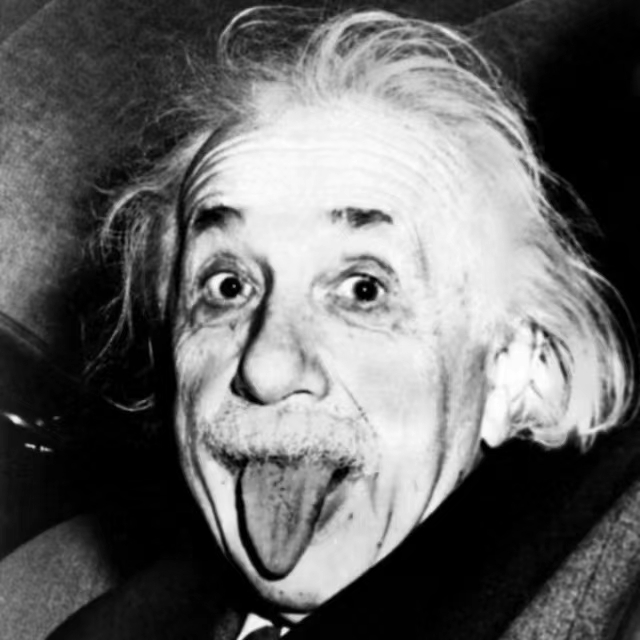
\includegraphics[width=2.8in]{Figures/mbti04-intp}% 
		\label{fig_text_feature_ablation}}
	\hfil
	\subfloat[]{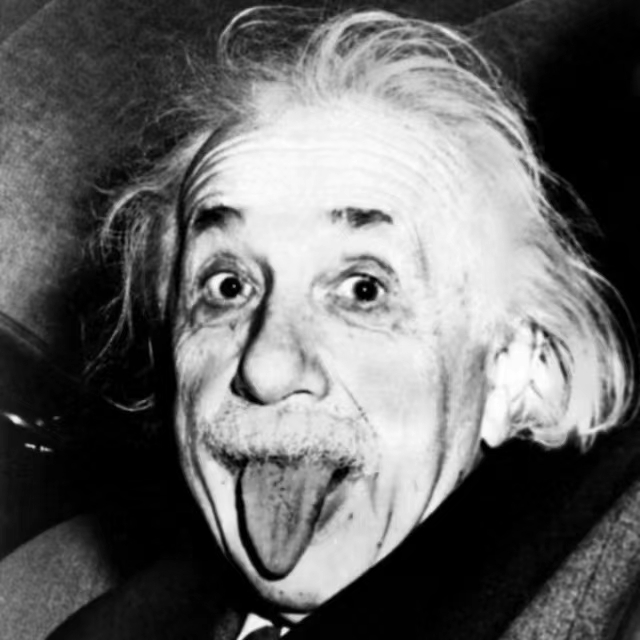
\includegraphics[width=2.8in]{Figures/mbti04-intp}
		\label{fig_visual_feature_ablation}}
	\bicaption{Lxx表现}{LMxxre ablation}
	\label{fig:feature ablation}
\end{figure*}


写点东西写点东西写点东西写点东西写点东西写点东西写点东西写点东西写点东西写点东西写点东西写点东西写点东西写点东西写点东西写点东西写点东西写点东西写点东西写点东西写点东西写点东西写点东西写点东西写点东西写点东西写点东西写点东西写点东西写点东西写点东西写点东西写点东西写点东西写点东西写点东西写点东西写点东西写点东西写点东西写点东西写点东西写点东西写点东西写点东西写点东西写点东西写点东西写点东西写点东西写点东西写点东西写点东西写点东西写点东西写点东西写点东西写点东西写点东西写点东西写点东西写点东西写点东西写点东西写点东西写点东西写点东西西写点东西写点东西写点东西写点东西写点东西写点东西写点东西写点东西写点东西写点东西写点东西写点东西写点东西写点东西写点东西写点东西写点东西写点东西写点东西写点东西写点东西写点东西写点东西写点东西写点东西写点东西写点东西写点东西写点东西写点东西写点东西写点东西写点东西写点东西写点东西写点东西写点东西写点东西写点东西写点东西写点东西写点东西写点东西写点东西写点东西写点东西写点东西写点东西写点东西写点东西写点东西写点东西写点东西写点东西写点东西写点东西写点东西写点东西写点东西写点东西写点东西写点东西写点东西写点东西写点东西写点东西写点东西写点东西写点东西写点东西写点东西写点东西写点东西写点东西写点东西点东西写点东西写点东西写点东西写点东西写点东西写点东西写点东西写点东西写点东西写点东西写点东西写点东西写点东西写点东西写点东西写点东西写点东西写点东西写点东西写点东西写点东西写点东西写点东西写点东西写点东西写点东西写点东西写点东西写点东西写点东西写点东西写点东西写点东西写点东西写点东西写点东西写点东西写点东西写点东西写点东西写点东西写点东西写点东西写点东西写点东西写点东西写点东西写点东西写点东西写点东西写点东西写点东西写点东西写点东西写点东西写点东西写点东西写点东西写点东西写点东西写点东西写点东西写点东西写点东西写点东西写点东西写点东西写点东西写点东西写点东西写点东西写点东西写点东西写点东西写点东西写点东西写点东西写点东西写点东西写点东西写点东西写点东西写点东西写点东西写点东西写点东西写点东西写点东西西写点东西写点东西写点东西写点东西写点东西写点东西写点东西写点东西写点东西写点东西写点东西写点东西写点东西写点东西写点东西写点东西写点东西写点东西写点东西写点东西写点东西写点东西写点东西写点东西写点东西写点东西写点东西写点东西写点东西写点东西写点东西写点东西写点东西写点东西写点东西写点东西写点东西写点东西写点东西写点东西写点东西写点东西写点东西写点东西写点东西写点东西写点东西写点东西写点东西写点东西写点东西写点东西写点东西写点东西写点东西写点东西写点东西写点东西写点东西写点东西写点东西写点东西写点东西写点东西写点东西写点东西写点东西写点东西写点东西写点东西写点东西写点东西写点东西写点东西写点东西点东西写点东西写点东西写点东西写点东西写点东西写点东西写点东西写点东西写点东西写点东西写点东西写点东西写点东西写点东西写点东西写点东西写点东西写点东西写点东西写点东西写点东西
写点东西写点东西写点东西写点东西写点东西写点东西写点东西写点东西写点东西写点东西写点东西写点东西写点东西写点东西写点东西写点东西写点东西写点东西写点东西写点东西写点东西写点东西写点东西写点东西写点东西写点东西写点东西写点东西写点东西写点东西写点东西写点东西写点东西写点东西写点东西写点东西写点东西写点东西写点东西写点东西写点东西写点东西写点东西写点东西写点东西写点东西写点东西写点东西写点东西写点东西写点东西写点东西写点东西写点东西写点东西写点东西写点东西写点东西写点东西写点东西写点东西写点东西写点东西写点东西写点东西写点东西写点东西西写点东西写点东西写点东西写点东西写点东西写点东西写点东西写点东西写点东西写点东西写点东西写点东西写点东西写点东西写点东西写点东西写点东西写点东西写点东西写点东西写点东西写点东西写点东西写点东西写点东西写点东西写点东西写点东西写点东西写点东西写点东西写点东西写点东西写点东西写点东西写点东西写点东西写点东西写点东西写点东西写点东西写点东西写点东西写点东西写点东西写点东西写点东西写点东西写点东西写点东西写点东西写点东西写点东西写点东西写点东西写点东西写点东西写点东西写点东西写点东西写点东西写点东西写点东西写点东西写点东西写点东西写点东西写点东西写点东西写点东西写点东西写点东西写点东西写点东西写点东西点东西写点东西写点东西写点东西写点东西写点东西写点东西写点东西写点东西写点东西写点东西写点东西写点东西写点东西写点东西写点东西写点东西写点东西写点东西写点东西写点东西写点东西





\vspace{12pt}
\begin{footnotesize}
	\begin{longtable}{|>{\columncolor{gray!15}}m{4cm}|m{1.7cm}<{\centering}|m{1.7cm}<{\centering}|m{1.7cm}<{\centering}|m{1.7cm}<{\centering}|}
		\bicaption{Top-3模xxTI对比}{Top-xxxtrue xxes}
		\label{fig:mbti case study}\\
		
		%表头
		\hline
		\endfirsthead
		

		% 表底
		\hline%\thickhline
		\endfoot
		
		\hline%\thickhline
		\endlastfoot
		
		% 第二组
		\hline\rowcolor{gray!15}
		\textbf{测试场景一} & \multicolumn{4}{c|}{\textbf{xxx}} \\ \hline
		\specialrule{0.75pt}{1pt}{0.5pt}\diagbox[dir=SE, width=4.4cm]{\textbf{xx}}{\textbf{xx}} & \raisebox{-.1\height}{\hspace{-1.5mm}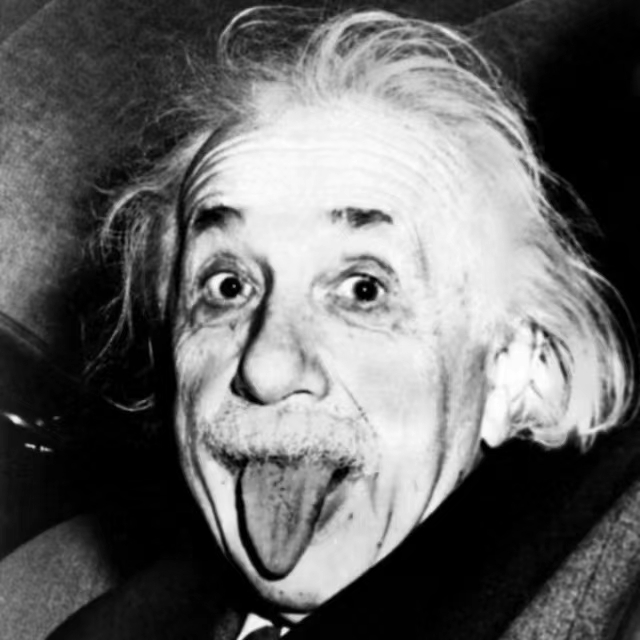
\includegraphics[width=2cm, keepaspectratio]{Figures/mbti04-intp}} & \raisebox{-.1\height}{\hspace{-1.5mm}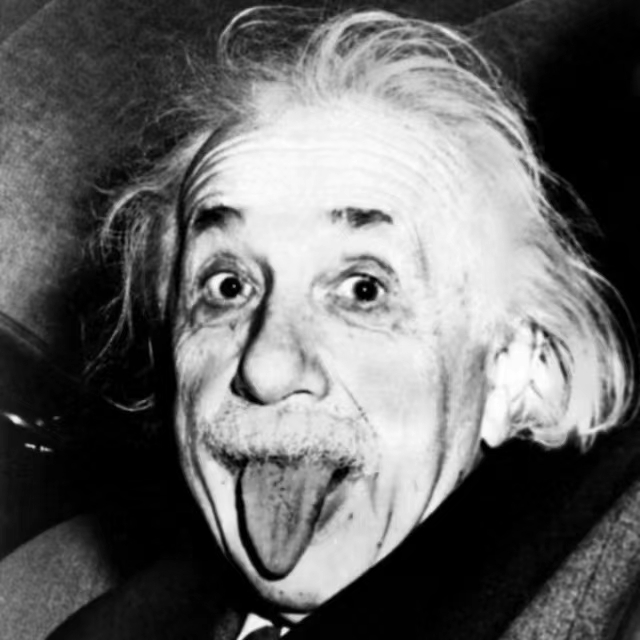
\includegraphics[width=2cm, keepaspectratio]{Figures/mbti04-intp}} & \raisebox{-.1\height}{\hspace{-1.5mm}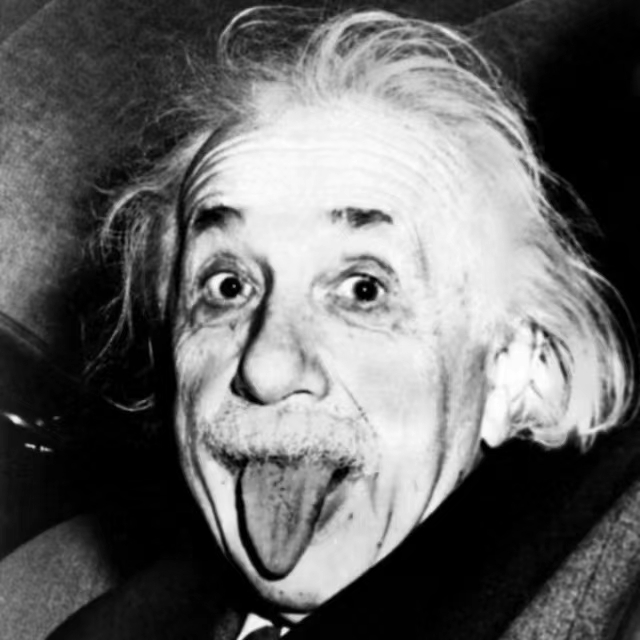
\includegraphics[width=2cm, keepaspectratio]{Figures/mbti04-intp}} & \raisebox{-.1\height}{\hspace{-1.5mm}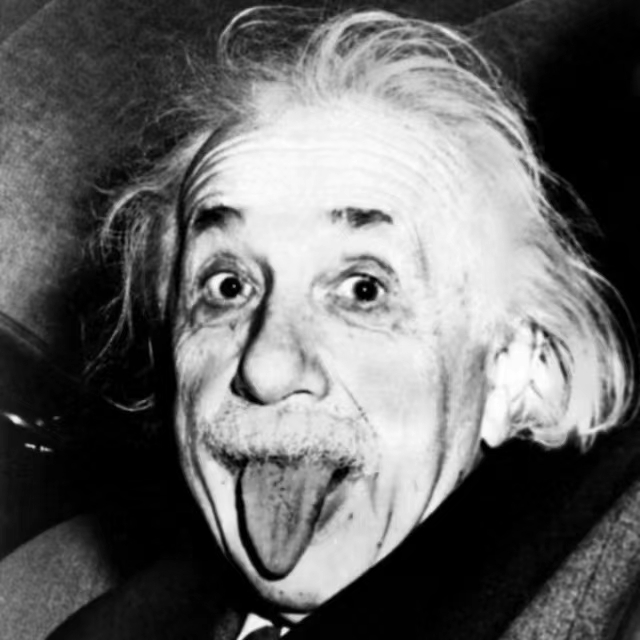
\includegraphics[width=2cm, keepaspectratio]{Figures/mbti04-intp}} \\
		\hline
		\specialrule{0.75pt}{1pt}{0.5pt}\cellcolor{white}\textbf{xxx} & \textbf{INFP} & \textbf{ENFP} & \textbf{ESTP} & \textbf{INTJ} \\
		\hline
		\cellcolor{white}xxx(ResNet Feature)
		& INF\textcolor{red}{J} & ENFP & E\textcolor{red}{N}TP & INTJ \\
		\hline
		\cellcolor{white}PM-xxx\cite{conferencekey} & INFP & ENFP & \textcolor{red}{IN}TP & I\textcolor{red}{S}TJ \\
		\hline
		\cellcolor{white}xxx\cite{conferencekey} & INF\textcolor{red}{J} & E\textcolor{red}{S}FP & E\textcolor{red}{N}T\textcolor{red}{J} & I\textcolor{red}{S}TJ \\
		\hhline{*{5}{:=}:}
		% 第三组
		\hline\rowcolor{gray!15}
		\textbf{测试场景二} & \multicolumn{4}{c|}{\textbf{单x拍}} \\ \hline
		\specialrule{0.75pt}{1pt}{0.5pt}\diagbox[dir=SE, width=4.4cm]{\textbf{测试模型}}{\textbf{xx}} & \raisebox{-.1\height}{\hspace{-1.5mm}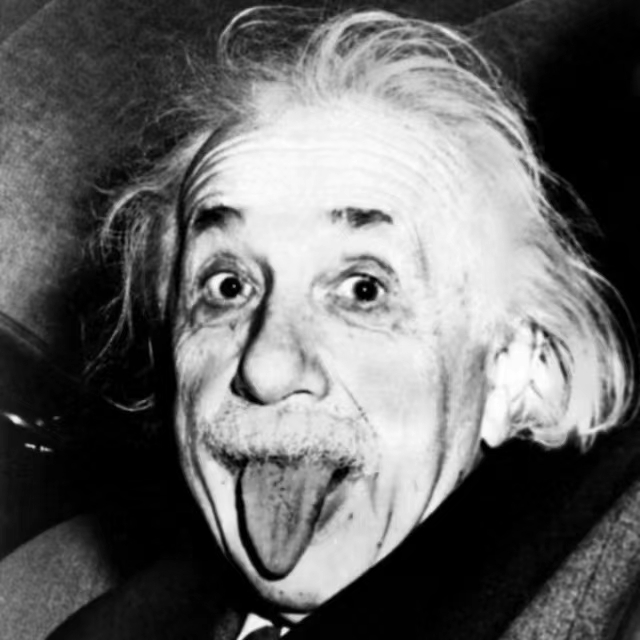
\includegraphics[width=2cm, keepaspectratio]{Figures/mbti04-intp}} & \raisebox{-.1\height}{\hspace{-1.5mm}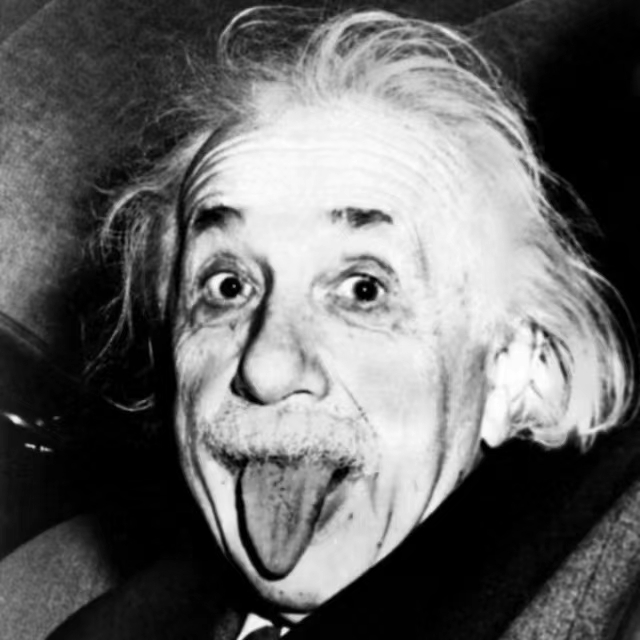
\includegraphics[width=2cm, keepaspectratio]{Figures/mbti04-intp}} & \raisebox{-.1\height}{\hspace{-1.5mm}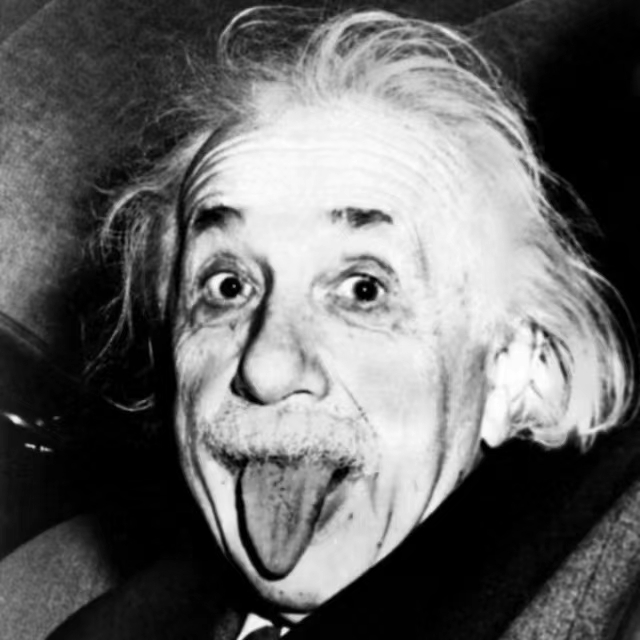
\includegraphics[width=2cm, keepaspectratio]{Figures/mbti04-intp}} & \raisebox{-.1\height}{\hspace{-1.5mm}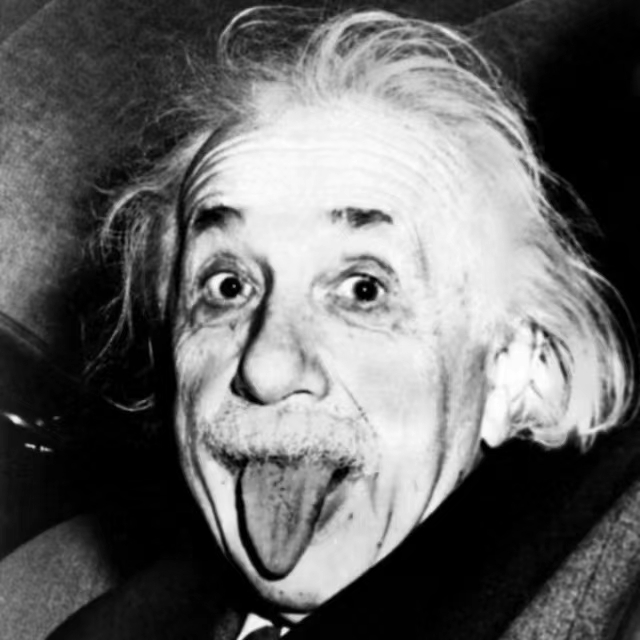
\includegraphics[width=2cm, keepaspectratio]{Figures/mbti04-intp}} \\
		\hline
		\specialrule{0.75pt}{1pt}{0.5pt}\cellcolor{white}\textbf{真实xTI} & \textbf{ISTJ} & \textbf{ISTJ} & \textbf{ISTJ} & \textbf{ISTJ} \\
		\hline
		\cellcolor{white}x(x Feature) & \textcolor{red}{ENF}J & \textcolor{red}{ENF}J & \textcolor{red}{E}S\textcolor{red}{F}J & \textcolor{red}{ENF}J \\
		\hline
		\cellcolor{white}PM-x\cite{conferencekey} & \textcolor{red}{ENF}J & \textcolor{red}{ENFP} & \textcolor{red}{E}S\textcolor{red}{FP} & I\textcolor{red}{NF}J \\
		\hline
		\cellcolor{white}xx\cite{conferencekey} & \textcolor{red}{ENFP} & \textcolor{red}{ENFP} & \textcolor{red}{ENF}J & \textcolor{red}{E}S\textcolor{red}{F}J \\
		%\hline
	\end{longtable}
\end{footnotesize}







\section{本章小结}

本章研究了x集。


